\section{What it learns}\label{sec:interp}

This section describes what v3's fitted members contain on the toy targets (\cref{sec:interp-toy}) and on images (\cref{sec:interp-img}). The analysis is descriptive: it says what structure the fits hold and when it appears, not why v3 does well, and nothing here is an ablation of the learner or a causal test. Every analysed fit is an instrumented seed-0 rerun of an evaluation fit, with the same training rows, column permutation and random streams. On the toy side every rerun reproduces the evaluation's seed-0 test error; on images, every rerun that has an evaluation cell reproduces it (\cref{app:interp-workflow}). Two independent verifiers per side checked the numbers and the readings, and their corrections are used throughout. Measured quantities are \status{Numerical}; descriptions of maps and explanations of mechanisms are \status{Heuristic}.

\paragraph{Findings.}
\begin{enumerate}
\item \emph{DFG finds the exact signed blocks} on 49 of the 54 sum-structured targets (median $n_{\rm struct}=256$), and its mean output then follows $E[f\mid t]$ level by level (\cref{sec:interp-toy-struct}).
\item \emph{Detection is cheap; discovery lags.} On the 25 pure symmetric targets the true block would pass DFG's test at $n=128$ every time. The delay to discovery tracks the share of variance at Fourier degrees 1--2 (Spearman $-0.86$), and the 10\% error point arrives with the block (\cref{sec:interp-toy-timing}). Since every seed of the block search starts from those statistics, this reads as the search, not the test, setting DFG's data cost \status{Heuristic}.
\item \emph{The residue classes mod 3 are never proposed.} They have $W_1+W_2\le0.0002$; the search's orders reach their block no better than chance and no piece of it carries signal, although at $n=16384$ the true block would pass the test at 134--155 times the threshold (\cref{sec:interp-toy-fail}).
\item \emph{Pooling sets and bars recover local pieces of the pixel grid.} On QuickDraw 98.3--99.9\% of the other members of a 4-pixel set lie within one step, and bars are short runs along recovered lines; on Fashion-MNIST 7\% of the 4-pixel sets include the mirror pixel (\cref{sec:interp-img-geom}).
\item \emph{The bar booster carries v3 on QuickDraw and MNIST.} \code{cgbt} has the lowest out-of-fold error of all 18 members in every analysed fit and takes \code{ggbt}'s stacking weight there; bars carry 0.77--0.80 of its split gain, 1.1--1.2 times their column share (\cref{sec:interp-img-members}).
\item \emph{Much class evidence lies on blank pixels}: 0.56--0.69 of \code{cgbt}'s net TreeSHAP evidence, often where other classes have ink, though per pixel inked pixels carry more on QuickDraw and MNIST (\cref{sec:interp-img-maps}).
\end{enumerate}
\Cref{app:interp-detail} has the per-target detail, the models below the discovery size and on the other suites, and the caveats; \cref{app:further-v2v3} says where v1.3's additions act in the fitted models.

% ==================================================================================================================
\subsection{Toy targets: the search, not the test, sets DFG's data cost}\label{sec:interp-toy}

On toy inputs v3 is a stack of DFG v1.3 (a default variant and, at $n\le512$, a forced small-$n$ variant) and the classical members (\cref{sec:portfolio}). The analysis looks at DFG's final model in each fit. It covers the 54 sum-structured targets of the six suites built around signed sums (\code{dlsymdev}, \code{dlfamdev}, \code{dlheld4}--\code{dlheld7}; the 14 non-symmetric controls are excluded) and, more briefly, the 70 targets of the other suites. The grid is $n=16,32,\dots,16384$, stopped after two consecutive sizes with test error $\le0.005$.

\paragraph{Definitions.}
\begin{itemize}
\item \emph{Terms and shares.} The model's terms are its characters, sum blocks (\cref{sec:dfg}), spectral features and the kernel background. A term's \emph{share} is the standard deviation of its contribution to the model's output over the 4096 test inputs.
\item \emph{Exact structure.} The target's signed-symmetry classes are the sets of inputs it treats alike, up to sign. A class of size $\ge3$ is \emph{matched exactly} when a sum block, a factor of a product block or the modulator $\chi_M$ of a modulated block has the same input set and the same signs up to a global flip. $n_{\rm struct}$ is the first grid size at which every class of size $\ge3$ is matched in the same model; we call it the \emph{discovery size}. For a weighted target $u=s+a\tau$ the class is the unit-weight part $s$; the inner term is checked separately (\cref{app:interp-forms}).
\item \emph{Detection.} $n_{\rm detect}$ is the first grid size at which DFG's own block test \eqref{eq:blocktest} would admit the \emph{true} block (the largest class, with its signs) if it were proposed in round 0 on the seed-0 training rows.
\item \emph{Reach.} The fraction of the true class $S$ among the first $|S|$ inputs of the better of the search's two eigenvector orders (\cref{fig:interp-toy-fail}a).
\item \emph{Low-degree share.} $W_k$ is the target's Fourier weight at degree $k$, and $(W_1+W_2)/(1-W_0)$ is the share of its variance at degrees 1 and 2.
\end{itemize}
The exact-structure criterion checks the input set and the signs, not the learned function of the block or its fold. It still tracks the function closely: at $n_{\rm struct}$ the DFG member's test error is at most 0.03 for every target found. It is also strict: some models fit a target exactly with another representation, and those count as not found (below). $n_{\rm detect}$ uses the true block, an oracle: it measures what the test would accept, not what the search would propose. For mixtures it is a rougher proxy, because DFG tests a block in later rounds on a residual from which the gate or parity characters are already fitted out (\cref{app:interp-mixtures}). Further caveats are in \cref{app:interp-below}.

\subsubsection{Exact structure}\label{sec:interp-toy-struct}

\begin{table}[tbp]
\centering{\footnotesize\setlength{\tabcolsep}{3.4pt}
\begin{tabularx}{\linewidth}{lrrrrrc>{\raggedright\arraybackslash}X}
\toprule
 & targets & \hd{exact\\structure} & \hd{median\\$n_{\rm struct}$} & \hd{range of\\$n_{\rm struct}$} & \hd{detectable\\at $n=128$} & \hd{delay (doublings)\\$<0$ / 0 / 1 / $\ge2$} & never found\\
\midrule
\multicolumn{8}{l}{\emph{by mixture}}\\
pure symmetric & 25 & 22 & 256 & 64--8192 & 25 & 1 / 9 / 3 / 9 & fd\_10, f7\_05, h6\_00\\
with a parity & 9 & 8 & 256 & 128--16384 & 9 & 0 / 3 / 3 / 2 & h6\_02\\
with a gate & 5 & 5 & 256 & 128--1024 & 0 & 2 / 3 / 0 / 0 & --\\
multiplexer & 4 & 3 & 512 & 512--1024 & 0 & 0 / 2 / 0 / 1 & f7\_11\\
two sums & 5 & 5 & 256 & 256--512 & 0 & 3 / 2 / 0 / 0 & --\\
weighted sum & 6 & 6 & 256 & 128--2048 & 5 & 0 / 1 / 3 / 2 & --\\
\addlinespace
\multicolumn{8}{l}{\emph{by accept set} (a two-block target counts once under each kind it has)}\\
threshold & 11 & 11 & 256 & 128--2048 & 7 & 2 / 3 / 4 / 2 & --\\
band & 19 & 18 & 192 & 64--1024 & 10 & 4 / 11 / 1 / 2 & f7\_11\\
interval & 10 & 9 & 256 & 128--1024 & 6 & 2 / 5 / 2 / 0 & h6\_02\\
arbitrary set & 16 & 15 & 512 & 128--16384 & 13 & 0 / 3 / 2 / 10 & f7\_11\\
residue class & 5 & 2 & 768 & 512--1024 & 3 & 0 / 1 / 0 / 1 & fd\_10, f7\_05, h6\_00\\
\addlinespace
all & 54 & 49 & 256 & 64--16384 & 39 & 6 / 20 / 9 / 14 & fd\_10, f7\_05, f7\_11, h6\_00, h6\_02\\
\bottomrule
\end{tabularx}
}
\caption{Exact structure in v3's DFG model on the 54 sum-structured targets, seed 0 \status{Numerical}. ``Exact structure'': targets whose model matches every signed-symmetry class of size $\ge3$ at some analysed $n$; $n_{\rm struct}$ is the first such $n$. ``Detectable at $n=128$'': the true block passes DFG's test \eqref{eq:blocktest} on the seed-0 training rows at $n=128$. For the five weighted targets other than sumpar the tested block is the weighted one, with v1.3's larger threshold. For the gate and multiplexer mixtures the detection points are the verifier's, recomputed with the residual deflated by the modulator as DFG tests it; the analysis file has 4 more targets at $n=128$. ``Delay'': $\log_2(n_{\rm struct}/n_{\rm detect})$ over the targets found. In the lower panel a target with two blocks counts once under each accept kind it has. Sources: \repo{study/part10/interp/tables/toy_timing.csv} and \repo{study/part10/interp/VERIFICATION.json}.}
\label{tab:interp-toy}
\end{table}

\paragraph{Exact structure is recovered on 49 of 54 targets} \status{Numerical}. \Cref{tab:interp-toy} gives the counts.
\begin{itemize}
\item \emph{When.} The median $n_{\rm struct}$ is 256 (range 64--16384). 15 targets have the exact structure by $n=128$, 30 by 256 and 41 by 512.
\item \emph{By suite.} \code{dlsymdev} 8 of 8, \code{dlfamdev} 8 of 9, \code{dlheld7} 7 of 9, \code{dlheld6} 7 of 9, \code{dlheld5} 10 of 10, \code{dlheld4} 9 of 9.
\item \emph{Never found} (by the largest analysed $n$; f7\_11's and h6\_02's runs stopped at 4096 and 1024 because the portfolio's error was already $\le0.005$): the three residue classes mod 3 of a 10--14-input count (fd\_10, h6\_00, f7\_05), and two targets that DFG fits by another representation. On f7\_11, a multiplexer between a 4-input and a 6-input block, each class is matched at some $n$ (128 and 2048), but never both in one model; at $n=4096$ the 4-input branch is carried by characters of degree 2--3. On h6\_02 $=[1\le s\le5]\,x_{10}x_{11}$, the model is a modulated block plus characters at $n=512$ (DFG error 0.002), and at $n=1024$ the degree-11 character on $x_1,\dots,x_{11}$ plus degree-3 characters.
\item \emph{Accept kinds.} Of the accept kinds learned on most of their targets, arbitrary sets need the most data (median 512; h5s7 8192, h5s1 16384). The only residue-class blocks that are learned are the 6-input multiplexer branches of f7\_03 (mod 4, $n=512$) and h6\_08 (mod 3, $n=1024$).
\end{itemize}

\paragraph{What the model looks like} \status{Numerical}. Where the structure is found, the leading terms take a few recurring forms: one block on the class with its signs (folded for accept sets symmetric under $t\to-t$) for pure targets, degree-1 characters beside the block for thresholds, a modulated block for a parity times a symmetric function, a product block for two sums, and gates and selectors as characters and, in v3, as the inner literal of a weighted block. The five weighted targets other than sumpar are fitted to DFG error 0 at their largest analysed $n$, two of them through exact product forms rather than the weighted block. \Cref{app:interp-forms} gives the examples and the inner terms.

\begin{figure}[tbp]
\centering
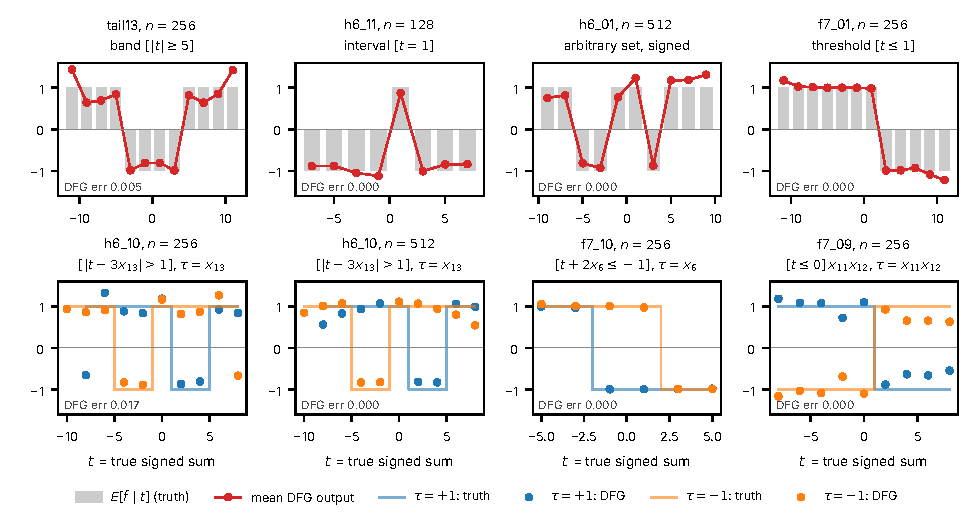
\includegraphics[width=\linewidth]{figures/fig_toy_g.pdf}
\caption{The learned function of the true block statistic $t$ (seed 0) \status{Numerical}. Top: grey bars are $E[f\mid t]$ over the 4096 test inputs; red points are the mean output of the whole DFG model at each level of $t$. Bottom: the same split by the second term $\tau$, from refits that reproduce the analysed cells. The plotted value is the conditional mean of the whole model, which includes spectral features, characters and stray product terms, not the block's own coefficients. Levels with fewer than 5 test points are not drawn; for h6\_10 at $n=256$ these include the cells $(t,x_{13})=(-10,+1)$ and $(10,-1)$, where the model is also wrong. ``DFG err'': the DFG member's test error. Source: the structure runs and \texttt{toy\_g} refits in \repo{study/part10/interp/results/toy_final/}.}
\label{fig:interp-toy-g}
\end{figure}

\paragraph{The learned function of the block} \status{Numerical} (\cref{fig:interp-toy-g}). Where the block is present, the model's mean output follows $E[f\mid t]$ level by level. This includes non-convex accept sets, such as h6\_01's $\{-9,-7,-5,-1,1,7,9\}$, and both branches of a weighted or modulated target. The values are not $\pm1$: the logistic readout rescales them and overshoots at rare extreme levels (tail13 at $|t|=11$). The panels add shape, not a new test. The share of test points at which the mean output has the sign of $E[f\mid t]$ is about one minus the DFG error by construction (0.983 for h6\_10 at $n=256$, 1.00 for the other seven panels). Below the discovery size the model has no block structure: for h6\_10 at $n=128$ the mean output is positive at every $(t,x_{13})$ level (0.01--0.90), so its sign agrees with $E[f\mid\cdot]$ only on the majority's 0.70 of the points, and the DFG error (0.39) is worse than a constant predictor's (0.30). The eight panels were chosen by hand; over all 53 exact cells of the 22 pure targets found, the agreement is at least 0.985 (\repo{study/part10/interp/VERIFICATION.json}, toy reading, C8).

\subsubsection{When the structure appears}\label{sec:interp-toy-timing}

\begin{figure}[tbp]
\centering
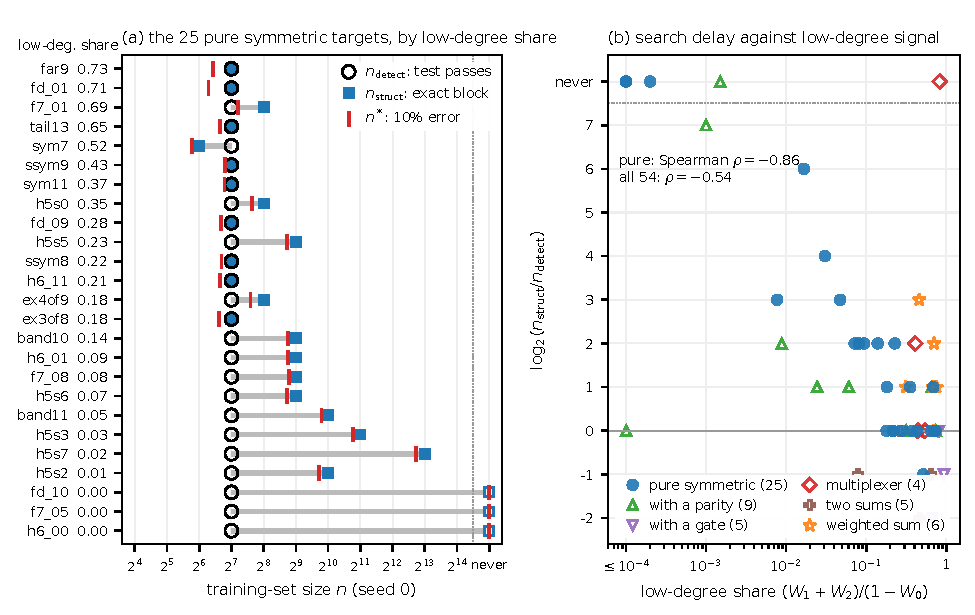
\includegraphics[width=\linewidth]{figures/fig_toy_timing.pdf}
\caption{When the structure appears (seed 0) \status{Numerical}. (a) The 25 pure symmetric targets, sorted by their share of variance at Fourier degrees 1--2 (number after the name). Open circle: $n_{\rm detect}$, the first grid size at which DFG's test would admit the true block. Square: $n_{\rm struct}$, the first grid size at which the model holds it exactly (open at ``never''); where $n_{\rm detect}=n_{\rm struct}$ the circle surrounds the square. Red tick: $n^*$, the 10\% test-error point of the same seed-0 fits, interpolated in $\log n$. The grey bar spans detection to discovery. (b) The delay $\log_2(n_{\rm struct}/n_{\rm detect})$ against the low-degree share for all 54 sum-structured targets; filled: pure symmetric, open: mixtures. Targets never found are drawn in the top row. Shares below $10^{-4}$ are drawn at $10^{-4}$, so h6\_00 and f7\_05 coincide at the top left. For the mixtures the detection points are the verifier's corrected ones (\cref{tab:interp-toy}). Spearman $\rho$ counts a target never found as $n_{\rm struct}=2^{15}$. No point is jittered. This figure replaces the analysis's \texttt{fig\_toy\_timing.pdf}, which used the uncorrected detection points. Sources: \repo{study/part10/interp/tables/toy_timing.csv} and \repo{study/part10/interp/VERIFICATION.json}.}
\label{fig:interp-toy-timing}
\end{figure}

\paragraph{Timing: the 25 pure symmetric targets} \status{Numerical}. On these targets the analysis is cleanest: the target is a function of one signed sum, and the round-0 test on the true block is close to the test DFG applies. \Cref{fig:interp-toy-timing}a shows each target.
\begin{itemize}
\item \emph{Detection is cheap.} The true block passes DFG's test at $n=128$ for all 25 targets. The test statistic grows linearly in $n$: its ratio to the threshold is at most 0.89 at $n=64$ and 1.07--1.78 at $n=128$.
\item \emph{Discovery is later where the low-degree signal is weak.} 22 of the 25 are found. Against $n_{\rm detect}$, $n_{\rm struct}$ is one doubling earlier for 1 target (sym7, held by the forced variant below the threshold), equal for 9, one doubling later for 3, and two or more later for 9 (band11, f7\_08, h6\_01, h5s2, h5s3, h5s5, h5s6, h5s7, band10).
\item \emph{The delay tracks the low-degree share} (\cref{fig:interp-toy-timing}b). Spearman's $\rho$ between the delay and $(W_1+W_2)/(1-W_0)$ is $-0.86$ over the 25 targets (a target never found counted as $n_{\rm struct}=2^{15}$), and $-0.80$ over the 22 found. The targets come from a few designed families, so a $p$-value that treats them as independent draws would overstate the evidence.
\item \emph{The readout is not the bottleneck.} For all 22 targets found, the seed-0 $n^*$ falls in the doubling just below $n_{\rm struct}$: the test error crosses 10\% between the last grid size without the exact block and the first with it. Because $n_{\rm struct}$ is a grid point and $n^*$ is interpolated, a finer statement cannot be made. In particular, the median offset of $\log_2(n^*/n_{\rm struct})$ ($-0.35$ over all 49 targets found) reflects the grid, not the readout.
\end{itemize}
\emph{Reading} \status{Heuristic}. For a function of one signed sum, DFG's data cost is set by its search, not by its test and not by its readout. Every seed of the block search reads the block's inputs off degree-1 and degree-2 statistics of the residual: prefixes of the top eigenvectors of the pair matrix, the degree-1 order and greedy growth from strong pairs (\cref{sec:dfg}). The weaker those statistics, the more data the search needs before it proposes the block, although the test would accept the block much earlier. No intervention isolates the search (such as seeding it with the true block); acceptance in later rounds and the stacker's choice of variant could also contribute.

\paragraph{The 29 mixtures} \status{Numerical}. For targets with a parity, gate, selector or second block, the round-0 test on the true block is a cruder proxy. With the verifier's corrected detection points (the modulated block tested on a residual already fitted on its modulator, as DFG tests it), 39 of the 54 targets are detectable at $n=128$, the median delay over the 49 found is 0 doublings, and Spearman's $\rho$ between delay and low-degree share over all 54 is $-0.54$ (\cref{app:interp-mixtures}).

\subsubsection{Where DFG fails: no low-degree foothold}\label{sec:interp-toy-fail}

\begin{figure}[tbp]
\centering
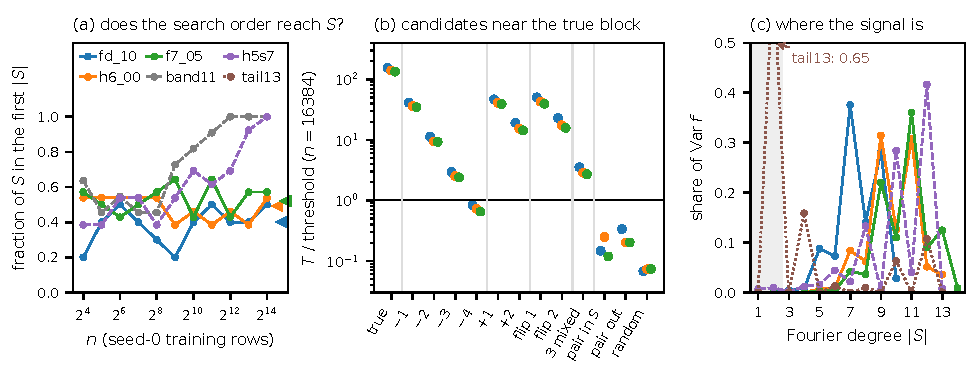
\includegraphics[width=\linewidth]{figures/fig_toy_failures.pdf}
\caption{Why the residue classes mod 3 are never found (seed-0 training rows) \status{Numerical}. (a) The fraction of the true class $S$ among the first $|S|$ inputs of the better of the search's two eigenvector orders. Triangles at the right edge: the value expected from the better of two random orders (0.40, 0.49, 0.52 for $|S|=10,13,14$). band11 and h5s7 are dashed (h5s7 also in (c)); they are found at the first $n$ at which all of $S$ lies within the order's first $|S|+5$ inputs (plotted fraction 0.82 and 0.92). The legend of (a) also serves (b) and (c). (b) DFG's test statistic over its threshold at $n=16384$ for the true block and for candidates near it: medians over 200 random candidates with 1--4 inputs dropped, 1--2 added, 1--2 signs flipped, or 3 errors of mixed kinds; the best 2-input block inside $S$; the best pair among 12 inputs outside $S$; random blocks of the true size. Above 1 the candidate passes. (c) The share of each target's variance by Fourier degree; degrees 1--2 shaded. tail13, found at $n=128$, has 0.65 at degree 2 (clipped). A compact version of the analysis's \texttt{fig\_toy\_failures.pdf}, with the chance level of panel (a) corrected for the better of two orders. Sources: \texttt{power/} and \texttt{toy\_landscape/} in \repo{study/part10/interp/results/toy_final/}.}
\label{fig:interp-toy-fail}
\end{figure}

\paragraph{The failures: residue classes mod 3} \status{Numerical}. Let $B=(s+k)/2$ count the $k$ signed inputs of the block that equal $+1$. Then fd\_10 $=[B\bmod3=0]$ on $k=10$ inputs, h6\_00 $=[B\bmod3\ne1]$ on 13 and f7\_05 $=[B\bmod3\ne0]$ on 14. Neither v3 nor v2 learns them (\cref{sec:res-toy-fail}). \Cref{fig:interp-toy-fail} shows why the search does not find them.
\begin{itemize}
\item \emph{The model.} At every $n\ge1024$ (fd\_10 from 128, f7\_05 from 256) the DFG model is the constant plus the kernel background. Its test error at $n=16384$ (0.32--0.34) is the test set's minority rate. For fd\_10 and h6\_00 these errors come from out-of-fold DFG fits on 13107 rows, which the stacker gave no weight. At smaller $n$ the forced variant adds 1--2 spurious characters or a spurious partial block (h6\_00 at $n=256$: $|-x_4+x_{12}-x_{22}-x_{23}|$, 2 of its 4 inputs in $S$).
\item \emph{The test would accept the block.} The true block passes from $n=128$ unfolded (512 folded). At $n=16384$ it is 155, 139 and 134 times the threshold.
\item \emph{There is no low-degree signal.} For h6\_00 and f7\_05, $W_1=W_2=0$ to five decimals; for fd\_10, $W_1=4\times10^{-5}$ and $W_2=1.7\times10^{-4}$. The Fourier weight peaks at degrees 7, 9 and 11.
\item \emph{The search's orders do not reach the block} (\cref{fig:interp-toy-fail}a). At $n=16384$ the eigenvector orders put 0.50, 0.54 and 0.57 of $S$ among their first $|S|$ inputs, against 0.40, 0.49 and 0.52 for the better of two random orders, and the fraction does not grow with $n$.
\item \emph{The basin is narrow} (\cref{fig:interp-toy-fail}b). At $n=16384$ the statistic falls about $4\times$ per missing input (to 41, 36 and 35 times the threshold with one input dropped; 2.9, 2.5 and 2.4 with three; 0.84, 0.73 and 0.65 with four). The first wrong sign or extra input costs $3.1$--$3.4\times$, the second $2.2$--$2.7\times$. Every sampled candidate with three errors of mixed kinds still passes. But no piece of the block carries signal: the best pair inside $S$ is at 0.15, 0.25 and 0.12 of the threshold, at the level of the best pair among 12 inputs outside $S$ (0.33, 0.20, 0.20), and random blocks of the true size are at 0.07. The basin estimate rests on medians of sampled candidates; other 4-error mixes were not measured.
\item \emph{A needle.} Within three errors of the true block there are $\sum_{j\le3}2^j\binom{30}{j}=34281$ candidates, against $\binom{30}{k}2^{k-1}=1.5\times10^{10}$, $4.9\times10^{11}$ and $1.2\times10^{12}$ blocks of the true size $k=10,13,14$.
\end{itemize}
\emph{Reading} \status{Heuristic}. A residue class mod 3 of a 10--14-input count is detectable once proposed and invisible from every low-order foothold the search has. For h6\_00 and f7\_05 the single and pair statistics are zero in expectation, so more data cannot help the seeds. For fd\_10 they are about 0.002, which the seeds could resolve only at $n$ of order $10^6$.

\paragraph{Late targets} \status{Numerical}. The pure targets found late, band11, h5s2, h5s3 and h5s7 (found at 1024--8192, with $W_1+W_2$ between 0.007 and 0.047), and h5s1, whose bottleneck is detecting its modulating parity, are consistent with the same mechanism in weaker form; h6\_08 and sumpar are late for representational reasons. Each is one seed (\cref{app:interp-late}).

% ==================================================================================================================
\subsection{Images: what the boosters split on}\label{sec:interp-img}

The analysis covers v3 on \code{qd_dev} at $n=1000$, 3000 and 10000, on \code{qd_a}, MNIST and Fashion-MNIST at $n=10000$, and v2 on \code{qd_dev} at $n=10000$. All four sets are development data for v3 (the held-out image sets are \code{qd_c} and \code{qd_d}), so the error comparisons below are in-sample; the held-out comparison is in \cref{sec:res-img-gain}. v2's analysis fit has test error 0.1467 against its multi-threaded evaluation cell's 0.1463 (\cref{sec:disc-provenance-disclosures}).
\begin{itemize}
\item \emph{Which booster is analysed.} The final \code{ggbt} and \code{cgbt} of each fit. On \code{qd_a} and MNIST the stacker gave \code{ggbt} weight 0, so it was not refitted, and the booster analysed is its out-of-fold fit on 8000 (7998) rows.
\item \emph{Geometry.} It is measured on the true $28\times28$ grid, which the learner never sees; for QuickDraw the columns are mapped back through the stored permutation. Distances are Chebyshev steps, so the 8 neighbours of a pixel are 1 step away.
\end{itemize}

\subsubsection{Pooling sets and bars on the true grid}\label{sec:interp-img-geom}

\begin{table}[tbp]
\centering{\footnotesize\setlength{\tabcolsep}{3.6pt}
\begin{tabular}{llrrrrrrrr}
\toprule
 & & \multicolumn{4}{c}{pooling sets: members other than $i$} & \multicolumn{2}{c}{Isomap $R^2$} & \multicolumn{2}{c}{bars: exact lines}\\
\cmidrule(lr){3-6}\cmidrule(lr){7-8}\cmidrule(lr){9-10}
set & $n$ & \hd{$S_i(4)$\\$\le1$ step} & \hd{$S_i(9)$\\$\le1$ step} & \hd{$S_i(9)$\\$\le2$ steps} & \hd{$S_i(9)$\\$>2$ steps} & \hd{$k=4$\\union} & \hd{$k=9$\\mutual} & $L=2$ & $L=4$\\
\midrule
\code{qd_dev} & 1000 & 0.983 & 0.823 & 0.985 & 79 & 0.84 & 0.87 & 0.33 & 0.16\\
\code{qd_dev} & 3000 & 0.991 & 0.829 & 0.991 & 46 & 0.97 & 0.89 & 0.38 & 0.21\\
\code{qd_dev} & 10000 & 0.994 & 0.834 & 0.994 & 31 & 0.97 & 0.92 & 0.42 & 0.24\\
\code{qd_a} & 10000 & 0.999 & 0.817 & 0.989 & 59 & 0.99 & 0.83 & 0.40 & 0.25\\
MNIST & 10000 & 0.976 & 0.787 & 0.966 & 186 & 0.92 & 0.97 & 0.20 & 0.06\\
Fashion & 10000 & 0.881 & 0.633 & 0.840 & 1006 & 0.13 & 0.23 & 0.11 & 0.04\\
\bottomrule
\end{tabular}
}
\caption{The pooling sets and bars of v3's image members on the true pixel grid (seed 0) \status{Numerical}. Pooling sets: the fraction of the $k-1$ members of $S_i(k)$ other than $i$ itself that lie within 1 or 2 Chebyshev steps of $i$, over all non-constant pixels $i$; ``$>2$ steps'': the number of such members (of 5408 on QuickDraw at $k=9$). Isomap $R^2$: Procrustes $R^2$ between a 2-D Isomap embedding of the pooling-set graph (an edge from $i$ to each member of $S_i(k)$; ``mutual'': only edges in both directions) and the true pixel coordinates. Bars: the fraction of bars of half-length $L$ whose pixels lie on one horizontal, vertical or diagonal lattice line. MNIST's $k=9$ mutual graph covers 674 of its 682 non-constant pixels. Source: the analysis files in \repo{study/part10/interp/results/image_final/v3/}.}
\label{tab:interp-img-geom}
\end{table}

\paragraph{Pooling sets are local neighbourhoods; on Fashion-MNIST some include the mirror pixel} \status{Numerical}. \Cref{tab:interp-img-geom} gives the geometry.
\begin{itemize}
\item \emph{QuickDraw.} 98.3--99.9\% of the other members of $S_i(4)$ lie within one step of $i$, and 98.5--99.4\% of those of $S_i(9)$ within two. Only 8 pixels lie within one step, so for $k=16$ at most $8/15=0.53$ of the other members can; 0.49 do. On \code{qd_dev} the members of $S_i(9)$ farther than two steps fall from 79 to 31 as $n$ grows from 1000 to 10000. The sets overlap the $k$ truly nearest pixels by 0.82, 0.88 and 0.78 for $k=4$, 9 and 16 at $n=10000$.
\item \emph{MNIST.} The 23 far members of $S_i(4)$ sit at 13 border pixels that are nonzero in at most 0.04\% of the 10000 training images. Their correlations rest on a handful of images.
\item \emph{Fashion-MNIST.} At 57 of the 784 pixels (7\%), $S_i(4)$ contains a far member, and all 65 far members are the centre's mirror pixel: the same row $\pm1$, with columns summing to $27\pm2$. At $k=9$, 619 of the 1006 far members are mirror pixels.
\end{itemize}
\emph{Reading} \status{Heuristic}. Garments are nearly left--right symmetric, so a pixel can correlate with its mirror image as strongly as with its neighbours. Sets at those pixels pool both sides of the garment.

\paragraph{The grid is recovered globally on QuickDraw and MNIST} \status{Numerical}. The 2-D Isomap embedding \cite{tenenbaum2000global} of the $k=4$ pooling-set graph matches the true grid with Procrustes $R^2$ 0.97--0.99 on QuickDraw at $n\ge3000$ (0.84 at $n=1000$), 0.92 on MNIST and 0.13 on Fashion-MNIST. Variants of the graph with a few long edges score much lower (\cref{app:interp-img-more}). The learner never builds a global embedding; it uses each set as a local sum. So $R^2$ summarizes how map-like the recovered neighbourhoods are, not a property the learner uses.

\begin{figure}[tbp]
\centering
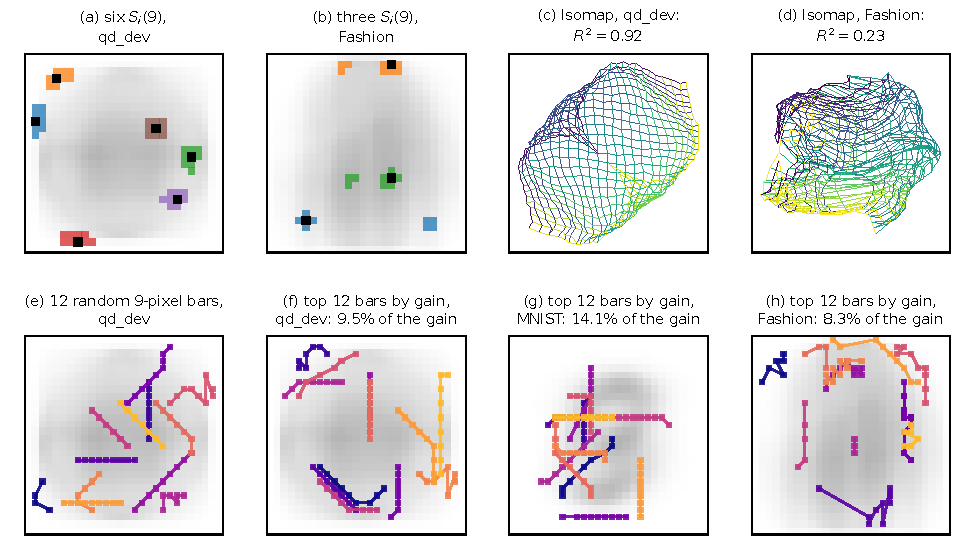
\includegraphics[width=\linewidth]{figures/fig_img_grid.pdf}
\caption{Pooling sets and bars of v3 on the true pixel grid, $n=10000$, seed 0 \status{Numerical}. Background: the average of the ten class-mean training images. (a) $S_i(9)$ at six pixels of \code{qd_dev} (black: $i$). (b) $S_i(9)$ at three inked Fashion-MNIST pixels whose sets contain mirror pixels. (c, d) The 2-D Isomap embedding of the $k=9$ mutual pooling-set graph, Procrustes-aligned to the grid and drawn as the true lattice: each pixel at its embedded position, joined to its horizontal and vertical grid neighbours (horizontal edges coloured by row, vertical edges by column). (e) Twelve randomly chosen 9-pixel bars ($L=4$) of \code{qd_dev}. (f--h) The twelve 9-pixel bars with the most split gain in \code{cgbt}, with their combined share of \code{cgbt}'s total gain. In (e)--(h) colour only distinguishes bars (in (f)--(h) darker means more gain); a bar's pixels are joined in order along its principal axis, so a long segment joins two separate pieces of one bar. Simplified from \texttt{fig\_img\_topology.pdf} and \texttt{fig\_img\_bars.pdf} in \repo{study/part10/interp/figures/}.}
\label{fig:interp-img-grid}
\end{figure}

\paragraph{Bars are short, nearly straight runs along recovered lines} \status{Numerical} (\cref{tab:interp-img-geom}, \cref{fig:interp-img-grid}).
\begin{itemize}
\item \emph{Shape on \code{qd_dev}.} At $n=10000$, 42\% of the 5-pixel bars ($L=2$) are exact lattice lines, and 96\% stay within one pixel of their principal axis. For the 9-pixel bars ($L=4$) the figures are 24\% and 63\%, since each further step can turn.
\item \emph{Growth with $n$.} The exact-line fraction grows with $n$ (0.33, 0.38, 0.42 for $L=2$ at $n=1000$, 3000, 10000; 0.16, 0.21, 0.24 for $L=4$). The within-one-pixel fraction does not, and it is a weak criterion for 5 pixels.
\item \emph{Orientation.} On QuickDraw all four orientations occur about equally often; on Fashion-MNIST horizontal and vertical bars dominate (0.37 and 0.40 at $L=2$).
\item \emph{Other sets.} On MNIST the bars are less straight (0.20 and 0.06 exact lines). On Fashion-MNIST they are rarely lines (0.11 and 0.04), and 27\% ($L=2$) and 30\% ($L=4$) contain a mirror pixel, against 2\% and 9\% on \code{qd_dev}. There a bar is often two short pieces on the two sides of the garment (\cref{fig:interp-img-grid}h).
\end{itemize}
Straightness is a property of the construction and the data, not of anything the booster learned.

\subsubsection{Which members carry v3}\label{sec:interp-img-members}

\begin{table}[tbp]
\centering{\footnotesize\setlength{\tabcolsep}{3.2pt}
\begin{tabular}{llrrrrrrrrrrr}
\toprule
 & & \multicolumn{6}{c}{share of the stacking weight} & \multicolumn{2}{c}{\hd{out-of-fold\\error}} & \multicolumn{3}{c}{test error}\\
\cmidrule(lr){3-8}\cmidrule(lr){9-10}\cmidrule(lr){11-13}
set & $n$ & \code{cgbt} & \code{ggbt} & \code{gknn} & \code{knn} & \hd{\code{gbt},\\\code{et}} & \code{lin_C} & \code{cgbt} & \code{ggbt} & stack & \hd{\code{cgbt}\\alone} & \hd{\code{ggbt}\\alone}\\
\midrule
\code{qd_dev} & 1000 & 0.32 & 0.09 & 0.44 & 0.16 & 0.00 & 0.00 & 0.272 & 0.280 & 0.2118 & 0.2208 & 0.2478\\
\code{qd_dev} & 3000 & 0.40 & 0.08 & 0.33 & 0.19 & 0.00 & 0.00 & 0.197 & 0.212 & 0.1753 & 0.1851 & 0.1968\\
\code{qd_dev} & 10000 & 0.47 & 0.07 & 0.17 & 0.25 & 0.03 & 0.00 & 0.149 & 0.161 & 0.1330 & 0.1368 & 0.1578\\
\code{qd_a} & 10000 & 0.56 & 0.00 & 0.15 & 0.24 & 0.06 & 0.00 & 0.161 & 0.172 & 0.1422 & 0.1442 & 0.1654$^a$\\
MNIST & 10000 & 0.40 & 0.00 & 0.23 & 0.24 & 0.13 & 0.00 & 0.031 & 0.043 & 0.0255 & 0.0278 & 0.0392$^a$\\
Fashion & 10000 & 0.10 & 0.16 & 0.00 & 0.04 & 0.50 & 0.20 & 0.126 & 0.127 & 0.1238 & 0.1216 & 0.1222\\
\addlinespace
v2, \code{qd_dev} & 10000 & -- & 0.41 & 0.24 & 0.24 & 0.11 & 0.00 & -- & 0.161 & 0.1467 & -- & --\\
\bottomrule
\end{tabular}
}
\caption{Which members carry v3 on images (seed 0, one fit each) \status{Numerical}. Left: each member family's share of the total stacking weight. \code{gknn}: $k$-NN votes on pooled sums; \code{knn}: $k$-NN votes on pixels; \code{gbt}, \code{et}, \code{lin_C}: Part 8's LightGBM, ExtraTrees and logistic regression on pixels. Middle: out-of-fold error of the two boosters (5-fold at $n\le3000$; one holdout of 2000 rows at $n=10000$). Right: test error of the stacked learner (v3; v2 in the last row) and of each booster alone (its own argmax). $^a$\code{ggbt} had stacking weight 0, so the booster shown is its out-of-fold fit on 8000 (\code{qd_a}) or 7998 (MNIST) rows; only the out-of-fold comparison is like for like there. Last row: v2's analysis fit. The weights are not shares of the decision (see the cautions in the text). Source: the analysis files in \repo{study/part10/interp/results/image_final/}.}
\label{tab:interp-img-stack}
\end{table}

\paragraph{\code{cgbt} is the member that carries v3 on QuickDraw and MNIST} \status{Numerical} (\cref{tab:interp-img-stack}).
\begin{itemize}
\item \emph{The best member.} \code{cgbt} has the lowest out-of-fold error of all 18 members in every v3 fit. The margin over \code{ggbt} is within holdout noise on Fashion-MNIST and at \code{qd_dev}, $n=1000$. It has the largest single-member weight everywhere except Fashion-MNIST, where Part 8's \code{gbt} has it.
\item \emph{Its weight.} Its share of the stacking weight grows with $n$ on \code{qd_dev} (0.32, 0.40, 0.47) and is 0.56 on \code{qd_a}, 0.40 on MNIST and 0.10 on Fashion-MNIST.
\item \emph{\code{ggbt} loses its weight.} At \code{qd_dev}, $n=10000$, \code{ggbt}'s share falls from 0.41 in v2's fit (0.37 in v2's evaluation cell) to 0.07 in v3. On \code{qd_a} and MNIST it is 0.
\item \emph{The rest of the weight.} Most of it goes to the $k$-NN members, on pooled sums and on pixels. On Fashion-MNIST half goes to Part 8's \code{gbt} and \code{et} and a fifth to logistic regression.
\item \emph{Alone.} On the test set \code{cgbt} alone beats \code{ggbt} alone on QuickDraw and MNIST (on \code{qd_a} and MNIST against \code{ggbt}'s out-of-fold fit on fewer rows; the like-for-like out-of-fold errors, 0.161 against 0.172 and 0.031 against 0.043, point the same way): 13.68\% against 15.78\% at \code{qd_dev}, $n=10000$. The two agree on 89--98\% of test points. The stack is 0.2--1.0 points better than \code{cgbt} alone on QuickDraw and MNIST; the 0.2 points on \code{qd_a} are not resolved by the test set. On Fashion-MNIST the stack (12.38\%) is not better than either booster alone (12.16\%, 12.22\%), a difference the test set does not resolve either.
\end{itemize}
Three cautions apply to the stacking weights, here and in \cref{tab:img-stack}.
\begin{itemize}
\item They act on log-probabilities of different calibration. Boosters stopped early on error give over-confident log-probabilities (clipped at $10^{-5}$), while $k$-NN votes, ExtraTrees and logistic regression are smoother. Equal weights are not equal influence.
\item The convex stacker splits weight between two nearly collinear boosters on one 2000-row holdout, so ``\code{ggbt} gets weight 0'' describes one fit. The 8 held-out fits at $n\ge10000$ show the same shift (\cref{sec:res-img-gain}).
\item The out-of-fold errors at $n=10000$ rest on those 2000 rows. Unpaired, the standard error of an error near 0.15 is about 0.008; for two members on the same rows the paired one is smaller.
\end{itemize}

\begin{table}[tbp]
\centering{\footnotesize\setlength{\tabcolsep}{4pt}
\begin{tabular}{lrrrrrr}
\toprule
 & \multicolumn{4}{c}{\code{cgbt}} & \multicolumn{2}{c}{\code{ggbt}}\\
\cmidrule(lr){2-5}\cmidrule(lr){6-7}
feature type & \code{qd_dev} & \code{qd_a} & MNIST & Fashion & \code{qd_dev} & Fashion\\
\midrule
pixels & 0.01 (0.1) & 0.01 (0.1) & 0.01 (0.1) & 0.09 (1.0) & 0.04 (0.1) & 0.16 (0.7)\\
pooled sums, $k=4$ & 0.02 (0.3) & 0.03 (0.3) & 0.05 (0.6) & 0.10 (1.1) & 0.10 (0.4) & 0.15 (0.7)\\
pooled sums, $k=9$ & 0.04 (0.5) & 0.05 (0.5) & 0.07 (0.9) & 0.10 (1.2) & 0.16 (0.7) & 0.16 (0.7)\\
pooled sums, $k=16$ & 0.15 (1.8) & 0.12 (1.5) & 0.07 (0.8) & 0.12 (1.4) & 0.32 (1.5) & 0.15 (0.6)\\
bars, $L=2$ & 0.24 (0.7) & 0.25 (0.8) & 0.30 (0.9) & 0.25 (0.7) & -- & --\\
bars, $L=4$ & 0.53 (1.6) & 0.54 (1.6) & 0.51 (1.5) & 0.35 (1.1) & -- & --\\
prototype pairs & -- & -- & -- & -- & 0.39 (4.1) & 0.38 (4.4)\\
\addlinespace
all bars & 0.77 (1.2) & 0.79 (1.2) & 0.80 (1.2) & 0.60 (0.9) & -- & --\\
all pooled sums & 0.22 (0.9) & 0.20 (0.8) & 0.19 (0.8) & 0.31 (1.3) & 0.57 (0.9) & 0.46 (0.7)\\
\midrule
columns & 8220 & 8220 & 8286 & 9408 & 3112 & 3436\\
\bottomrule
\end{tabular}
}
\caption{Split gain by feature type in the final boosters, $n=10000$, seed 0 \status{Numerical}. Each entry is the type's share of the booster's total split gain, with its ratio to the type's share of the columns in brackets (1.0: as much gain per column as the booster's average). Bars are two thirds of \code{cgbt}'s columns; the 300 prototype pairs are about a tenth of \code{ggbt}'s. LightGBM samples 5\% (\code{cgbt}) or 12\% (\code{ggbt}) of the columns per tree. \code{ggbt} on \code{qd_a} and MNIST, an out-of-fold fit, is not shown (pairs 0.30 and 0.41 of its gain). Split gain describes how the trees split, not what the predictions depend on. Source: the analysis files in \repo{study/part10/interp/results/image_final/v3/}.}
\label{tab:interp-img-gain}
\end{table}

\paragraph{Split gain by feature type} \status{Numerical} (\cref{tab:interp-img-gain}).
\begin{itemize}
\item \emph{The bars in \code{cgbt}.} The bars carry 0.77--0.80 of \code{cgbt}'s split gain on QuickDraw and MNIST at $n=10000$ (0.72 at \code{qd_dev}, $n=1000$) and 0.60 on Fashion-MNIST. They are two thirds of its columns, so this is 1.1--1.2 times their column share (0.9 on Fashion-MNIST): more than their share, not dominance. They also make 0.75 of the splits at \code{qd_dev}, $n=10000$. Per column, the 9-pixel bars (1.5--1.6; 1.1 on Fashion-MNIST) and, on QuickDraw, the 16-pixel pooled sums (1.5--1.8) carry the most. The 5-pixel bars carry 0.7--0.9 of the average, and single pixels 0.1, except on Fashion-MNIST (1.0).
\item \emph{The pairs in \code{ggbt}.} The 300 prototype pairs carry about 0.4 of \code{ggbt}'s gain (0.30 in \code{qd_a}'s out-of-fold fit), about four times their column share. On \code{qd_dev} the 16-pixel pooled sums come next (1.5).
\item \emph{Use is wide, gain concentrated.} Almost every bar is split on at least once (at \code{qd_dev}, $n=10000$: 2520 and 2596 of 2704 for $L=2$ and 4). But the top 10\% of bars carry 0.65--0.66 of the bar gain there (0.76 at $n=1000$), 0.78--0.84 on Fashion-MNIST and 0.86 on MNIST. The twelve 9-pixel bars with the most gain carry 9.5\%, 14.1\% and 8.3\% of \code{cgbt}'s total gain on \code{qd_dev}, MNIST and Fashion-MNIST (\cref{fig:interp-img-grid}f--h).
\end{itemize}

\paragraph{v3 against v2 at \code{qd_dev}, $n=10000$} \status{Numerical}. The two fits have identical pooling sets and a bit-identical \code{ggbt}: the same gain vector, test predictions and maps, and 123 rounds in both. So, as far as checked, the fits differ by \code{cgbt}, the stacking weights, and which members are refitted. The errors are 0.1467 for v2 and 0.1330 for v3. 2.08\% of the test points are right in v3 and wrong in v2, and 0.71\% the reverse. Per-class detail is in \cref{app:interp-v2}.

\subsubsection{Class evidence maps}\label{sec:interp-img-maps}

\paragraph{Class evidence maps: method and limits.} For each class, 100 test points of that class are taken. LightGBM's TreeSHAP contributions \cite{lundberg2020local} of each feature to that class's raw score are computed and spread over pixels. A pixel keeps its own contribution. A pooled sum or bar spreads its contribution equally over its pixels. A prototype pair $u=x_a-x_b$ spreads it over pixels $j$ in proportion to $|u_jx_j|$. The maps are averaged over the 100 points. They can show where in the image the features that raise a class's score look. They cannot show more than that, for five reasons.
\begin{itemize}
\item \emph{Own score only.} A map is the contribution to the class's own raw score in a 10-class softmax, not to its margin over the other classes.
\item \emph{No causal test.} Nothing was occluded or ablated, so no region is shown to be necessary.
\item \emph{The spreading rule.} Spreading a subset sum equally over its pixels books part of the evidence of a partly inked bar on blank pixels. On \code{qd_dev}, of the members of bars with at least one inked member, 43\% ($L=2$) and 52\% ($L=4$) are blank. So evidence on blank pixels marks where a feature looks, not necessarily what drove it.
\item \emph{Built-in agreement.} The pairs' maps follow the class's own ink by construction. \code{cgbt} and \code{ggbt} share the pixels, the pooled sums and the spreading rule, so part of their agreement is built in.
\item \emph{Post-hoc regions.} The regions named in the Reading and in \cref{app:interp-maps-ex} were drawn after looking at the maps. Their shares describe the maps; they do not test them.
\end{itemize}

\begin{figure}[tbp]
\centering
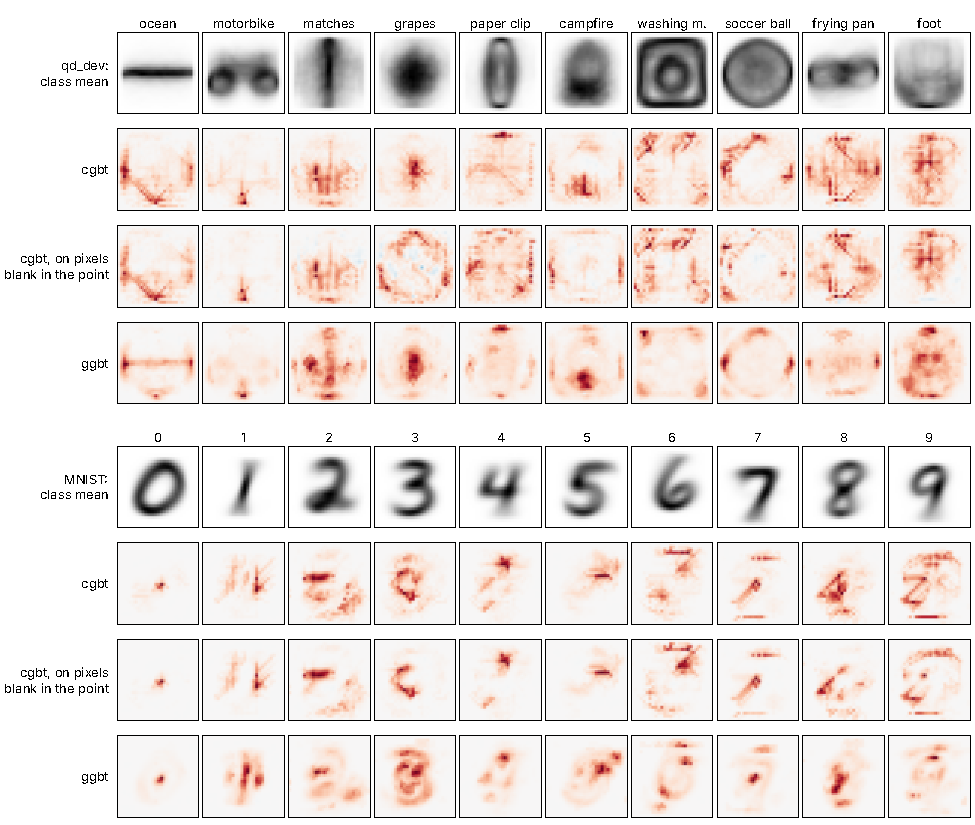
\includegraphics[width=\linewidth]{figures/fig_img_contrib.pdf}
\caption{Class evidence maps of v3's two boosters on \code{qd_dev} and MNIST, $n=10000$, seed 0 \status{Numerical}. Each map is the mean, over 100 test points of the class, of the TreeSHAP contributions to that class's own raw score, spread over pixels as described in the text; red is positive, and each map is scaled to its own 99th percentile of $|$value$|$ (the top 1\% saturate). Rows: the class's mean training image; \code{cgbt}; the part of \code{cgbt}'s map on pixels blank in the point ($x\le0.1$); \code{ggbt}, prototype pairs included. The maps are descriptive (see the text for what they cannot show). Simplified from \texttt{fig\_img\_contrib\_qd\_dev.pdf} and \texttt{fig\_img\_contrib\_mnist.pdf} in \repo{study/part10/interp/figures/}, which also show the pooled-sum and pair parts, and Fashion-MNIST and \code{qd_a}.}
\label{fig:interp-img-contrib}
\end{figure}

\paragraph{What the maps show} \status{Numerical} for the shares (\cref{fig:interp-img-contrib}).
\begin{itemize}
\item \emph{Sign.} The mean maps are almost all positive: positive values make at least 0.96 of each map's absolute mass.
\item \emph{Blank pixels.} The share of the net evidence on pixels blank in the point, averaged over classes, is 0.61 for \code{cgbt} on \code{qd_dev}, 0.56 on Fashion-MNIST, 0.69 on MNIST and 0.62 on \code{qd_a}. For \code{ggbt} it is 0.39--0.44, and 0.53--0.68 once its pairs are removed. Blank pixels are 0.75, 0.73, 0.83 and 0.55 of these images (\code{qd_dev}, \code{qd_a}, MNIST, Fashion-MNIST), so per pixel, inked pixels carry more of the evidence on QuickDraw and MNIST, and Fashion-MNIST is at par. It is not so for every class: grapes, soccer ball and campfire (0.32--0.39 on \code{qd_dev}), pullover, shirt and coat (0.25--0.29), camouflage on \code{qd_a} (0.15) and the digit 8 (0.42) draw most of their evidence from ink.
\item \emph{Agreement.} The \code{cgbt} and \code{ggbt} maps of a class correlate at 0.63--0.94 on \code{qd_dev}, Fashion-MNIST and MNIST, and at 0.40--0.88 on \code{qd_a} (slightly less over non-constant pixels only: 0.60--0.94 and 0.33--0.87).
\item \emph{By feature type.} By absolute contribution, \code{cgbt}'s evidence on \code{qd_dev} is 0.78 bars, 0.20 pooled sums and 0.02 pixels. \code{ggbt}'s is 0.64 pooled sums, 0.29 pairs and 0.07 pixels.
\end{itemize}
\emph{Reading} \status{Heuristic}. In these maps a sizable part of a class's evidence sits where the class has no ink and other classes do; for several digits the largest named region is an open one (0, 1, 3, 4, 7). Two examples (shares \code{cgbt} / \code{ggbt} of the class's net evidence): on MNIST the hole of the 0 carries 0.46 / 0.41 of the evidence on 3\% of the image, 99\% of it on blank pixels; on \code{qd_dev} the blank gap between a motorbike's wheels carries 0.20 / 0.16 (\cref{app:interp-maps-ex} lists the others). \code{cgbt} does not look at different places from \code{ggbt}. It looks at the same places through thinner, oriented windows: lines and chains of short segments, where \code{ggbt}'s pooled sums give blobs. That difference in shape follows from the feature shapes and is not learned. What the fit chose is which segments carry weight.
